\documentclass[border=3pt]{standalone}
% Preâmbulo compartilhado pelos diagramas TikZ da aula 4 de Navegação (Representação de Mapas)
\usepackage[T1]{fontenc}
\usepackage[utf8]{inputenc}
\usepackage{lmodern}
\usepackage{amsmath}
\usepackage{xcolor}
\usepackage{tikz}
\usetikzlibrary{arrows.meta,angles,quotes,decorations.pathmorphing,decorations.pathreplacing,calc,
                positioning,shapes.geometric,shapes.misc,backgrounds,fit,
                math}

% Paleta (mesma dos SVGs originais)
\definecolor{dblue}{HTML}{2A5B8C}
\definecolor{dorange}{HTML}{B3541E}
\definecolor{dgreen}{HTML}{4A7C59}
\definecolor{dred}{HTML}{9C4B4B}
\definecolor{dcream}{HTML}{F4F1EA}
\definecolor{dshade}{HTML}{DDD7C9}

% Função gaussiana (não normalizada por padrão de escala visual)
\pgfmathdeclarefunction{gauss}{3}{%
  \pgfmathparse{1/(#3*sqrt(2*pi))*exp(-((#1-#2)^2)/(2*#3^2))}%
}

% Estilos comuns (prefixo d... para não colidir com chaves internas do pgf)
\tikzset{
  >={Stealth[length=2mm]},
  dguide/.style={gray!55, dashed, line width=0.4pt},
  daxis/.style={gray!60, line width=0.7pt, ->},
  dbody/.style={fill=black!3, draw=black!80, line width=1pt},
  dacc/.style={draw=dblue, line width=1pt},
  dlbl/.style={black!55, font=\small},
  dsub/.style={black!45, font=\footnotesize},
  dstate/.style={circle, draw=black!80, fill=dcream, line width=1pt,
                 minimum size=17mm, font=\large, inner sep=1pt},
  dobs/.style={circle, draw=black!80, fill=dshade, line width=1pt,
               minimum size=14mm, font=\large, inner sep=1pt},
  dbox/.style={rounded corners=2pt, draw=black!80, fill=dcream, line width=1pt,
               align=center, inner sep=6pt},
  dop/.style={circle, draw=black!80, fill=white, line width=1pt,
              minimum size=6mm, inner sep=0pt, font=\small},
  dtrans/.style={->, dblue, line width=1pt},
  dmeas/.style={->, dorange, line width=1pt},
  dcurve/.style={line width=1pt, dblue},
  dcurveb/.style={line width=1.4pt, dorange},
}

\begin{document}
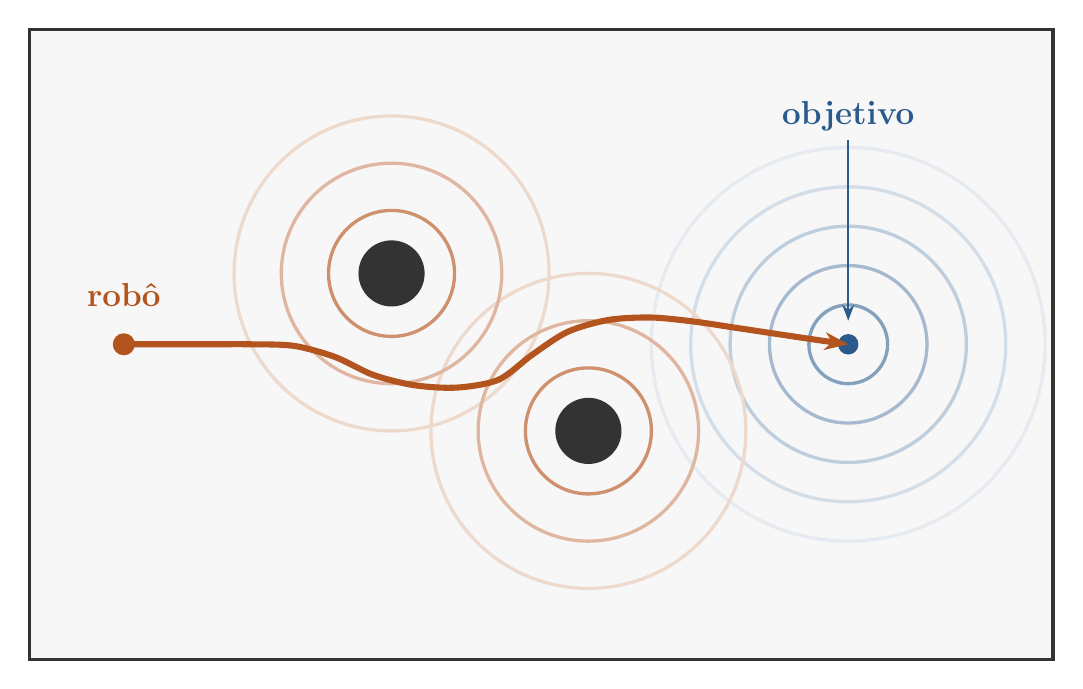
\begin{tikzpicture}[x=1cm,y=1cm]

  \draw[dbody, line width=1.2pt] (0,0) rectangle (13,8);

  \coordinate (goal) at (10.4,4.0);
  \coordinate (obsA) at (4.6,4.9);
  \coordinate (obsB) at (7.1,2.9);
  \coordinate (start) at (1.2,4.0);

  % Campo atrativo do objetivo (círculos convergentes)
  \foreach \r/\o in {2.5/12,2.0/20,1.5/30,1.0/42,0.5/58} {
    \draw[dblue!\o!white, line width=1.2pt] (goal) circle (\r);
  }
  % Campo repulsivo dos obstáculos: alcance 2,0 (mais forte perto)
  \foreach \r/\o in {2.0/22,1.4/42,0.8/65} {
    \draw[dorange!\o!white, line width=1.2pt] (obsA) circle (\r);
    \draw[dorange!\o!white, line width=1.2pt] (obsB) circle (\r);
  }
  \fill[black!80] (obsA) circle (0.42);
  \fill[black!80] (obsB) circle (0.42);
  \fill[dblue] (goal) circle (0.13);
  \node[dblue, font=\large\bfseries] at (10.4,6.9) {objetivo};
  \draw[dblue, line width=0.8pt, -{Stealth[length=2mm]}] (10.4,6.6) -- (10.4,4.3);

  % Caminho: descida do gradiente do campo (atração constante + repulsão de alcance 2,0)
  \draw[dorange, line width=2.2pt, -{Stealth[length=3mm]}] plot[smooth] coordinates {(1.20,4.00) (1.74,4.00) (2.28,4.00) (2.82,4.00) (3.36,3.98) (3.88,3.84) (4.37,3.61) (4.89,3.48) (5.43,3.45) (5.96,3.55) (6.39,3.87) (6.84,4.16) (7.36,4.31) (7.90,4.34) (8.43,4.29) (8.97,4.21) (9.50,4.13) (10.04,4.05) (10.40,4.00)};
  \fill[dorange] (start) circle (0.14);
  \node[dorange, font=\large\bfseries, anchor=south] at (1.2,4.35) {robô};

\end{tikzpicture}
\end{document}
